%\begin{figure}
%	\begin{center}
%		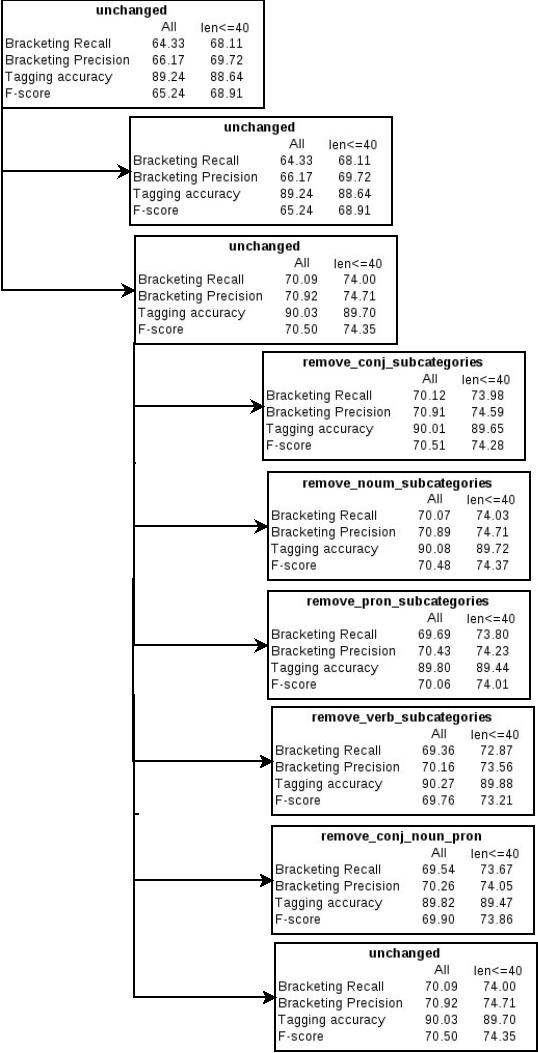
\includegraphics[scale=0.35]{diagrama_experimentos1.jpeg}
%		\caption{\label{evolucao} Evolução dos resultados }		
%	\end{center}
%\end{figure}

Na execução dos experimentos inicialmente trabalhamos sobre a influêcia da escolha do núcleo \emph{(Head)} dos constituíntes que é essencial na implementação dos algorítmos de implementação dos modelos propostos por Collins \cite{collins99}.

O corpus do Bosque ja tem anotados muitos dos \emph{heads} das sentenças disponibilizadas, porém o parser de bikel precisa de todos os \emph{heads}, e verificou-se que nem todas as sentenças possuem essa informação, tendo que ser analisada e construída de forma empírica.

A ferramenta de Bikel possibilita a utilização de um módulo para especificação de regras para determinar o \emph{head} de um constituinte e optou-se por se usar esse módulo e construir regras baseadas nas regras de formação da lingua portuguesa incrementalmente (já exemplificado em capítulo anterior). 

\subsection{Configurações}
\label{sec:configuracoes}

A primeira estratégia abordada foi quanto as regras de definição do núcleo das sentenças. Serão experimentadas quatro configurações.

A primeira configuração utilizada foi a default para o inglês, com regras de definição do núcleo especificas para o PTB, a segunda configuração de definição do núcleo foi a utilização das regras básicas, ou seja, o núcleo da sentença é a primeira palavra da direita para a esquerda, regra essa que é padrão na lingua inglesa, para terceira configuração se alterou as regras para que o núcleo da sentença seja a primeira palavra da esquerda para a direita, regra que ja se aproxima da regra de formação da lingua portuguesa. Para a quarta e última configuração desta bateria de experimentos foi definido regras de definição do núcleo das sentenças baseados na construção das sentenças para a lingua portuguesa.

É interessante mensionar que a construção das regras foi incremental e experimentos paralelos com um conjunto menos de sentenças foram sendo feitos apenas para avaliar a qualidade das regras criadas.

O corpus utilizado tambem sofreu um processo incremental de avaliação, utilizou-se primeiramente o corpus apenas com as categorias de POS sintáticas principais, nesse experimento foi feito o agrupamento de TAGS que possuem subgrupos dentro da mesma categoria.

O último conjunto de regras utilizado é o que estamos usando atualmente, bem melhor que o original conforme resultados apresentados. Acreditamos que não teremos ganho nos resultados tentando melhorar as regras de head-find, e sim se ajustarmos melhor os parâmetros da ferramenta.

Para a segunda configuração de testes foi eleito a configuração vencedora como partida, usamos as configurações para o português definidas por Dan Bikel em seu parser e com as regras de de definição do núcleo das sentenças que atingiram melhor resultado.

A estratégia nessa segunda bateria de testes é avaliar a separação das TAGS de POS em subgrupos. A ideia básica é que tags devem ser distintos quando a categorias tem distribuições sintáticas diferentes, por outro lado se duas classes tem mesma distribuição ou distribuição próxima, separa-las apenas levará a perda de qualidade quanto a informação sintática constante nas sentenças, esse tipo de configuração também será observado na evolução dos experimentos.

Para avaliar o efeito da distinção de categoria verbal em diferentes distribuições, primeiro será feito a distinção dos verbos que inicialmente foi testado apenas sob a TAG V, agora será avaliado as suas subcategorias VFIN, VINF, VPCP, VGER. Logo será feito avaliado com a TAG PRON e suas subcategorias PRONPERS PRONINDP, com a TAG CONJ e duas subcategorias CONJC e CONJS 


Removendo subcategorias de verbo separadamente...
Removendo subcategorias de conjução separatamente...
Removendo subcategorias de pronomes separadamente...
Removendo subcategorias de substantivo separadamente...

Removento todas as sub categorias das TAGS na qual possuem sub categorias. 

\subsection{Dificuldades}
\label{sec:dificuldades}

Uma das grandes dificuldades encontradas neste trabalho, foi com relação aos verbos. No português as inflexões verbais são significativamente mais complexas. Os verbos são conjugados em seis pessoas e em dez tempos com representação morfológica diferente, além de em diversas formas não finitas. Além disso muitas terminações de verbos são idênticas aos sufixos flexionais ou derivacionais usados para formar substantivos, isso complica e muito a tarefa de análise morfológica. Dificuldade esta também relatada por Wing e Baldridge em seu trabalho.

Verificou-se conforme esperado que para verbos é bastante relevante as sub-categorias pois a distribuição sintática das diferentes categorias verbais é bem distinta, da mesma forma para pronomes porque os possessivos tem diferente distribuição que os pessoais; os .. tem posição de pré-modificadores nominal e os outros ...

Diferenciando conjunçao coordenada e subordinativa nao houve diferença significativa nos resultados.

O último caso relativo a nomes refere-se  o que ... do corpus 

Foi dada grande atenção quando ao tratamento das palavras desconhecidas pois acreditamos que um ajuste nesse ponto se pode alcançar desempenhos melhores.

Quanto ao idioma, cada pacote de idioma também pode ser codificado com base nas características morfológicas de uma palavra, estas são especificamente importantes para palavras desconhecidas. Cinco características são codificadas para cada palavra, capitalização, hifenização, numérico, inflexão e derivação. Os três primeiros indicam respectivamente se as palavras estão capitalizadas contém hífem ou estão sob forma de número. Para a maior parte, o código para crialos não precisou mudanças. Já para os dois últimos ítens tivemos que fazer modificações para trabalhar corretamente com o português. Pois como falado anteriormente, inflexões verbais e derivações no português são os grandes problemas.


\subsection{Experimentos com lematização das palavras}
\label{sec:lematizacao}

Como experimento mais avançado foram feitos testes utilizado lematização das palavras do corpus, primeiro com todas as palavras das sentenças, logo apenas com os verbos. A fim de verificar a qualidade do treino executado pela ferramenta de Bikel.

Um analisador sintáxico automático permite resolver corretamente as ambiguidades ligadas à sintaxe. Ao aplicar-se as
regras gramaticais à frase e às proposições que a compõem, pode-se, na maioria dos casos, diferenciar verbos,
substantivos, adjetivos e substitui-los pela sua forma canônica (singular de um substantivo, infinitivo de um verbo por
exemplo), mas também identificar as palavras compostas e as locuções. Esse trabalho aplicado ao texto se chama
lematização.

Em Linguística, lematização é o processo de agrupar as diferentes formas flexionadas de uma palavra para que possam ser analisados como um único item.

No português, palavras aparecem em várias formas flexionadas. Por exemplo, o verbo 'caminhar' pode aparecer como 'caminha', 'caminhado', 'caminhou'. A forma de base, 'caminhar', que se pode olhar em um dicionário, é chamado o lema para a palavra. A combinação da forma de base com a parte do discurso é muitas vezes chamada de lexema da palavra.

Lematização está intimamente relacionado com decorrentes. A diferença é que um derivado opera em uma única palavra, sem o conhecimento do contexto e, portanto, não pode discriminar entre palavras que têm significados diferentes dependendo da parte do discurso.

Para os experimentos realizados nesse trabalho, foi utilizado o lematizadorde palavras TreeTagger (Pablo Gamallo Otero , Grupo de Procesamento de Linguagem Natural da Universidade de Santiago de Compostela), que tem a função de receber uma palavra e retornar o lema e sua TAG.

A lematização dos verbos principalmente torna-se importante porque o português é uma lingua morfologicamente rica, onde um verbo pode aparecer em dezenas de formas,diferentemente do inglês. Acreditávamos que a lematização poderia contribuir para se atingir melhores resultados.




